\documentclass[a4paper,11pt]{article}
\usepackage[spanish]{babel}
\usepackage[utf8]{inputenc}

% Configuración páginas
\usepackage{vmargin}							% Márgenes

\usepackage{sectsty}							% Fuente de los títulos
\allsectionsfont{\normalfont \Large \scshape}

\usepackage{graphicx}							% Imágenes
\graphicspath{{images/}}

\usepackage{tabularx}							% Otras tablas
\usepackage{multirow}							% Celdas ocupando múltiples filas en tablas
\usepackage{listliketab}						% Tratar indentación distas como tablas

\usepackage{mathtools}							% Matematicas
\newcommand\numberthis{							% numeración en align*
	\addtocounter{equation}{1}\tag{\theequation}
}

% Configuración del título
\newcommand{\horrule}[1]{\rule{\linewidth}{#1}} 	% Horizontal rule

\title{
	\vspace{-25pt}
	\normalfont \Large \textsc{
		Modelos de Investigación Operativa,
        Ingeniería Informática\\
        Universidad de Valladolid
	}\\[10pt]
	\horrule{1pt}\\[10pt]
	\huge \textbf{
		Práctica 16
	}\\
	\horrule{1pt}
}
\author{
	\normalfont \Large Daniel González Alonso
}
\date{
	\normalfont \large \today
}

%%%%%%%%%%%%%%%%%%%%%%%%%%%%%%%%%%%%%%%%%%%%%%%%%%
\begin{document}
\maketitle

%%%% RESUMEN %%%%
\begin{abstract}
	En este documento se describen los problemas y los resultados obtenidos de la práctica 16 del tema 6 de la asignatura Modelos de Investigación Operativa de Ingeniería Informática, Universidad de Valladolid.
\end{abstract}

%%%% DESARROLLO %%%%
\section{Introducción}
Esta práctica, al igual que la práctica anterior, trata de problemas de Rutas de Vehículos Capacitado (CVRP, \textit{Capacited Vehicle Routing Problem}).\\


Tal y como se presentó en la práctica anterior, los problemas CVRP tratan determinar las rutas que una flota de vehículos ha de seguir con el fin de cubrir la demanda de todos sus clientes. Los datos del problema se representan como un grafo ${G=(V,A)}$, donde ${V}$ son los vértices del grafo, el primer vértice es el depósito de salida de los vehículos y el resto los clientes a a abastecer, y ${A}$ los arcos entre éstos, con un coste ${c_{i,j}}$ asociado a cada arco. Cada vértice del grafo tiene asociado una demanda ${d_{i} \geq 0}$, en el caso del depósito esta demanda es siempre ${d_{1}=0}$. Por otro lado, se supone que nuestra flota de vehículos es homogénea, es decir todos los vehículos tienen la misma capacidad, con un total de ${K}$ vehículos. También se supone que todos los puntos de demanda pueden ser satisfechos y que la matriz de costes satisface la desigualdad triangular:

\begin{align*}\numberthis
	\label{desigualdad_triangular}
	c_{i,k} + c_{k,j} \geq c_{i,j}	&& \forall i,j,k \in V \\
\end{align*}

Para poder resolver este problema en la presente práctica, se nos pide emplear el algoritmo de ahorros Clark-Wright, el cual consta de los siguientes pasos:

\begin{enumerate}
\item Calcular la matriz de ahorros (\textit{savings}): Para cada arco ${i}$ y nodo ${j}$ calculamos el ahorro que supondría incluir un arco ${(i,j)}$ en la ruta de la solución, el cual se calcula mediante la siguiente fórmula:

\begin{equation}
\label{saving}
s(i,j) = c_{1,i} + c_{j,1} - d_{i,j}
\end{equation}

\item Ordenamos los ahorros de mayor a menor.

\item Creamos una solución inicial: La solución inicial consta de un total de ${n-1}$ rutas conectando el vértice 1 (depósito) con cada vértice cliente.

\item Se recorre esta lista uniendo las rutas siempre que sea posible, es decir, siempre que cumplan las restricciones, como por ejemplo la capacidad de los vehículos.
\end{enumerate}

%%%%%%%%%%%%%%%%%%%%%%%%%%%%%%%%%%%%%%%%%%%%%%%%%%%%%%
\section{Desarrollo}
Para esta práctica se nos pide resolver una serie de problemas con distancias Euclídeas mediante el algoritmo Clarke-Wright y comparar la solución obtenida con la de los algoritmos exactos de la práctica anterior.\\

Los problemas en cuestión se encuentran en los ficheros \texttt{data/E021-04m.dat}, \texttt{data/E026 \ -08m.dat}, \texttt{data/E051-05e.dat} y \texttt{data/E076-10e.dat}. Todos estos problemas se resolvieron mediante \textit{Xpress Mosel} usando el modelo de flujo de redes en los ficheros \texttt{cvrp\_clarke \ \_wright\_e021.mos}, \texttt{cvrp\_clarke\_wright\_e026.mos}, \texttt{cvrp\_clarke\_wright\_e051.mos} y \texttt{cvrp \ \_clarke\_wright\_e076.mos} (el nombre indica el fichero de datos empleado).\\

Para la implementación de este problema lo primero que se tuvo que calcular, una vez cargados los datos, fue la matriz de costes a partir de las coordenadas empleando la distancia Euclídea redondeada al entero más cercano.\\

A continuación se implementó el algoritmo Clarke-Wright. En mi caso a la hora de ordenar los ahorros en el paso 2 del apartado anterior, creé una lista llamada \texttt{savings\_list} con los indices ${i}$ y ${j}$ de los vértices que uniría el posible arco. Para obtener el ahorro solo se tiene que indexar con estos índices en la matriz de ahorros \texttt{savings}. Por otro lado, para almacenar las diferentes rutas creé un total de ${n-1}$ matrices, una por cada ruta inicial, con los arcos de cada ruta. Además utilicé un vector llamado \texttt{rutas\_activas} para poder saber qué ruta ya había sido unida o descartada así como otro vector llamado \texttt{rutas\_demandas} con la demanda total de cada ruta. Así para implementar el último paso del algoritmo, solo se tendría que buscar 2 rutas activas, las cuales una empezara con un arco ${(1,j)}$, llamada \texttt{ruta\_i}, y otra acabara con un arco ${(i,1)}$, llamada \texttt{ruta\_j}. Si estas rutas existen, ${\texttt{ruta\_i} \neq \texttt{ruta\_j}}$ y además la demanda de ${\texttt{ruta\_i} + \texttt{ruta\_j} \leq \texttt{capacidad}}$ entonces se unirían las rutas.


%%%%%%%%%%%%%%%%%%%%%%%%%%%%%%%%%%%%%%%%%%%%%%%%%%%%%%
\section{Resultados}
Los resultados obtenidos a los anteriores problemas, junto con los gráficos IVE que representan los caminos de las soluciones (obtenidos a partir de las coordenadas de los ficheros de datos), son los siguientes:

\begin{table}[!htbp]
\label{results_e0}
\centering
\begin{tabularx}{\textwidth}{|X|X|X|X|X|}
\hline
Fichero de datos	& \texttt{E021-04m.dat}	& \texttt{E026-08m.dat}	& \texttt{E051-05e.dat}	& \texttt{E076-10e.dat}	\\ \hline
Nº de vértices	& 21	& 26	& 51	& 76	\\ \hline
Solución	& 391	& 626	& 582	& 889	\\ \hline
Nº de vehículos	& 5	& 9	& 6	& 11	\\ \hline
Valores de x (arcos)	& (1,2) (1,3) (1,5) (1,14) (1,21) (2,7) (3,6) (4,10) (5,16) (6,1) (7,13) (8,1) (9,1) (10,8) (11,19) (12,20) (13,18) (14,15) (15,9) (16,4) (17,1) (18,1) (19,17) (20,11) (21,12)	& (1,3) (1,4) (1,7) (1,8) (1,13) (1,16) (1,18) (1,21) (1,23) (2,24) (3,5) (4,1) (5,26) (6,1) (7,15) (8,12) (9,10) (10,1) (11,1) (12,9) (13,1) (14,17) (15,6) (16,20) (17,1) (18,2) (19,25) (20,1) (21,22) (22,14) (23,19) (24,1) (25,1) (26,11)	& (1,2) (1,16) (1,18) (1,28) (1,33) (1,48) (2,23) (3,17) (4,29) (5,19) (6,13) (7,1) (8,44) (9,49) (10,11) (11,50) (12,3) (13,47) (14,26) (15,1) (16,46) (17,39) (18,38) (19,1) (20,41) (21,36) (22,30) (23,21) (24,7) (25,1) (26,15) (27,8) (28,9) (29,32) (30,51) (31,35) (32,27) (33,12) (34,40) (35,22) (36,37) (37,4) (38,45) (39,6) (40,31) (41,42) (42,14) (43,20) (44,25) (45,43) (46,34) (47,1) (48,5) (49,24) (50,1) (51,10)	& (1,4) (1,7) (1,12) (1,18) (1,24) (1,48) (1,52) (1,53) (1,69) (1,73) (1,76) (2,74) (3,31) (4,45) (5,35) (6,30) (7,1) (8,27) (9,1) (10,40) (11,32) (12,66) (13,59) (14,55) (15,1) (16,58) (17,64) (18,13) (19,51) (20,36) (21,38) (22,29) (23,62) (24,57) (25,50) (26,56) (27,1) (28,16) (29,63) (30,1) (31,46) (32,26) (33,10) (34,3) (35,47) (36,9) (37,70) (38,6) (39,54) (40,41) (41,1) (42,43) (43,65) (44,42) (45,33) (46,1) (47,68) (48,37) (49,22) (50,1) (51,25) (52,17) (53,28) (54,8) (55,20) (56,19) (57,44) (58,14) (59,39) (60,15) (61,71) (62,1) (63,2) (64,34) (65,23) (66,67) (67,60) (68,1) (69,75) (70,72) (71,21) (72,61) (73,11) (74,1) (75,49) (76,5)	\\ \hline
\end{tabularx}
\caption{Resultados obtenidos para los ficheros \textit{e0}}
\end{table}

\begin{figure}[!htbp]
	\centering
	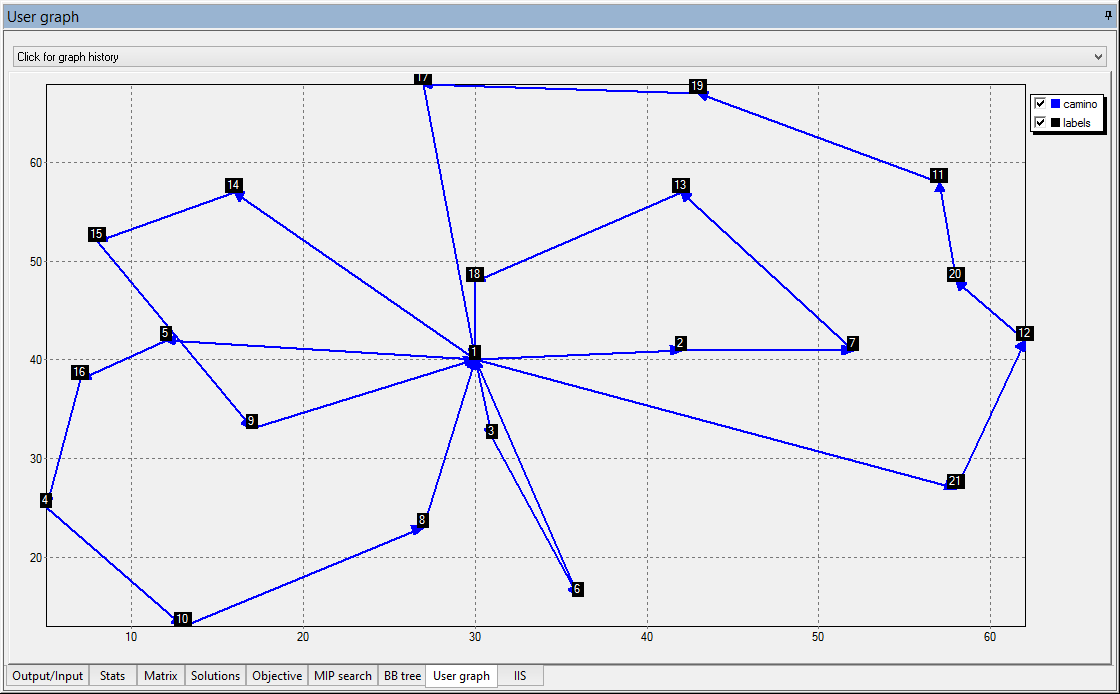
\includegraphics[width=1.0\textwidth]{e021_clarke_wright.png}
    \caption{Solución del problema \texttt{E021-04m.dat}}
\end{figure}

\begin{figure}[!htbp]
	\centering
	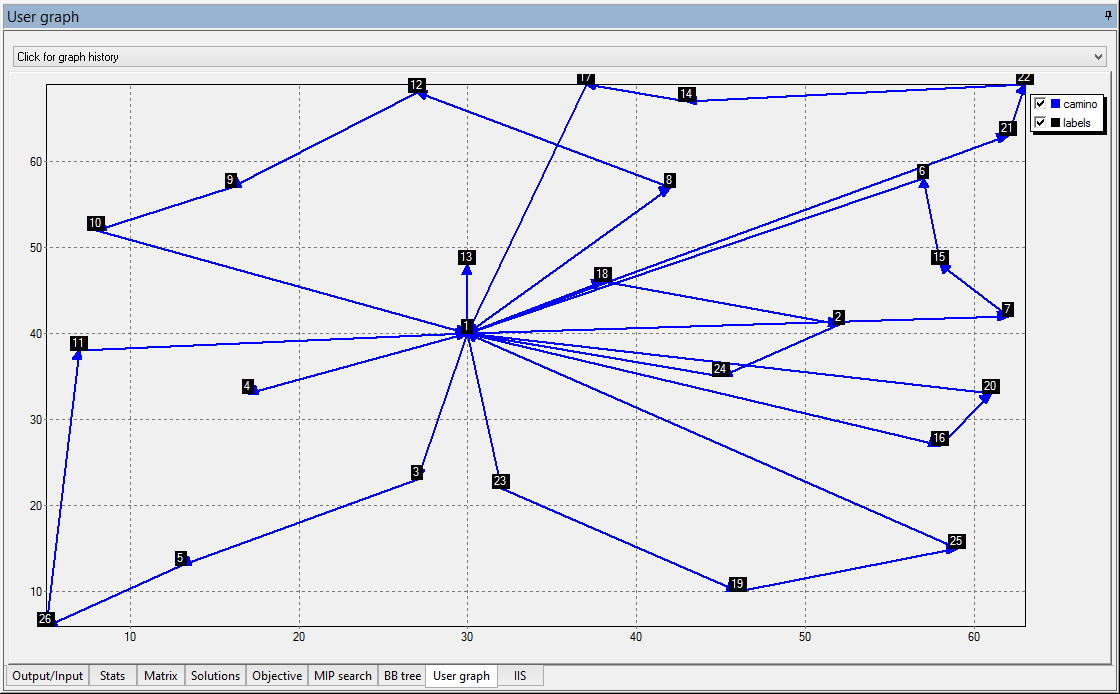
\includegraphics[width=1.0\textwidth]{e026_clarke_wright.png}
    \caption{Solución del problema \texttt{E026-08m.dat}}
\end{figure}

\begin{figure}[!htbp]
	\centering
	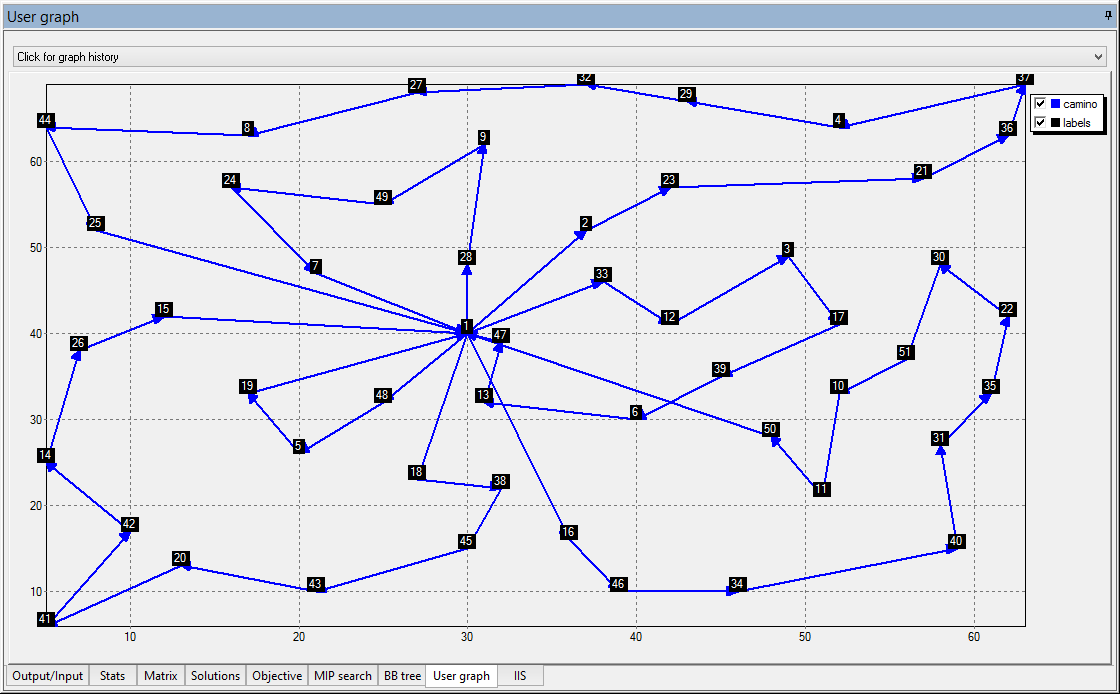
\includegraphics[width=1.0\textwidth]{e051_clarke_wright.png}
    \caption{Solución del problema \texttt{E051-05e.dat}}
\end{figure}

\begin{figure}[!htbp]
	\centering
	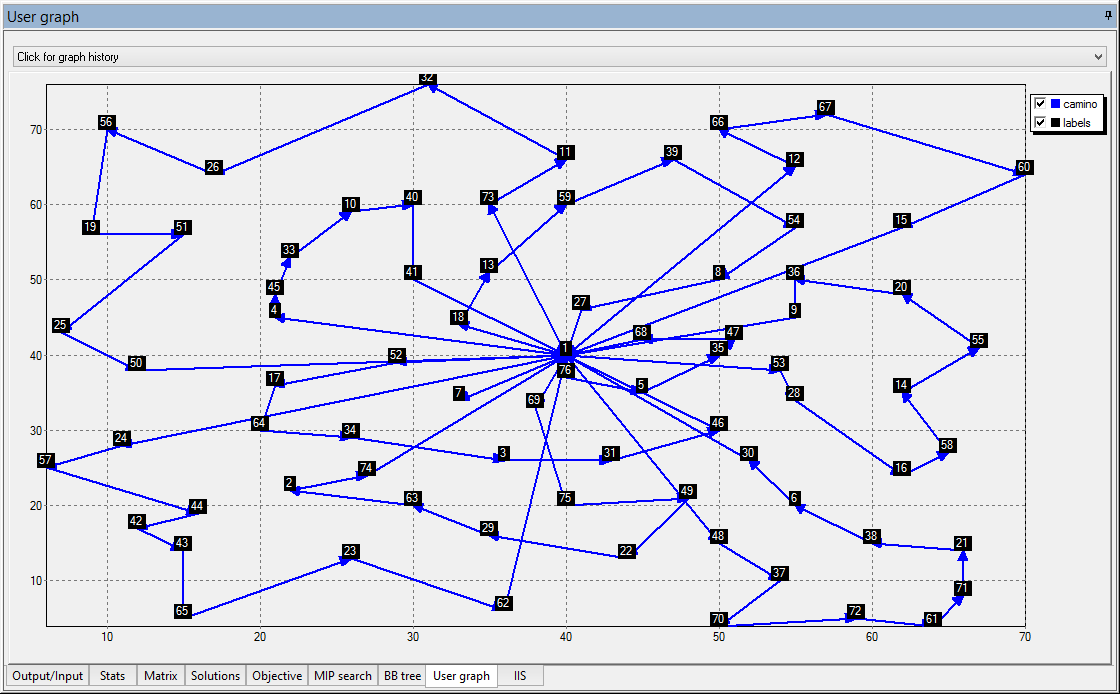
\includegraphics[width=1.0\textwidth]{e076_clarke_wright.png}
    \caption{Solución del problema \texttt{E076-10e.dat}}
\end{figure}

\clearpage
Por último, en la siguiente tabla se pueden comparar los resultados obtenido con el algoritmo exacto (modelo de flujo de redes) de la práctica 15 con los de la práctica actual:

\begin{table}[!htbp]
\label{results_e0}
\centering
\begin{tabularx}{\textwidth}{|X|X|X|X|X|X|}
\hline
\multicolumn{2}{|l|}{Fichero de datos}	& \texttt{E021-04m}	& \texttt{E026-08m}	& \texttt{E051-05e}	& \texttt{E076-10e}	\\ \hline
\multirow{3}{2cm}{Modelo de flujo de redes}	& Nº de vértices	& 21	& 26	& 51	& 76	\\ \cline{2-6}
											& Solución	& 358	& 606	& 584	& 918	\\ \cline{2-6}
											& Nº de vehículos	& 5	& 9	& 7	& 12	\\ \hline
\multirow{3}{2cm}{Algoritmo Clarke-Wright}	& Nº de vértices	& 21	& 26	& 51	& 76	\\ \cline{2-6}
											& Solución	& 391	& 626	& 582	& 889	\\ \cline{2-6}
											& Nº de vehículos	& 5	& 9	& 6	& 11	\\ \hline
\end{tabularx}
\caption{Comparación de resultados para los ficheros \textit{e0}}
\end{table}

Como se puede observar, el algoritmo exacto da mejores resultados para los dos primeros ficheros de datos, mientras que el algoritmo Clarke-Wright emplea menos vehículos y un menor coste para los dos últimos.

\end{document}
